\problemname{Forest Highway}

\illustration{.28}{frog.jpg}

The Slovak Government is building a highway from Bratislava to Košice. The highway will pass through
a forest where a lot of animals live. Frog Gizela, the queen of the animals, wants to calculate the
impact of the highway on their lives. Since the highway will be noisy, animals don't want to live
within distance $d$ from the highway. Gizela wants to know how large the inhabitable area will be.
If the total inhabitable area of the forest is too small, Gizela will have to find a new forest
for her kingdom.

\section*{Task}

You are given a description of the forest and the highway. The forest is a simple polygon, i.e.\ its
sides do not cross, and the highway can be considered a straight line of width zero. You are also
given $d$, the safe distance from the highway. Calculate the size of the inhabitable area of the forest.

\begin{figure}[h]
    \begin{center}
    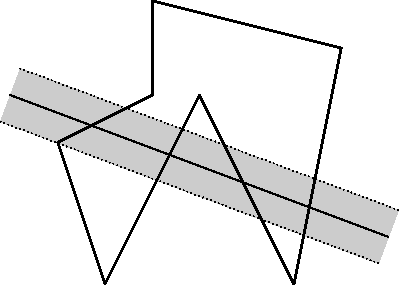
\includegraphics[width=0.44\textwidth]{polygon}
    \caption{Drawing of the sample input}
    \end{center}
\end{figure}

\section*{Input}
The first line of the input contains one integer $N$ $(3\leq N\leq 250\,000)$ denoting the number
of vertices of the polygon. $N$ lines follow with two floating point numbers $x_i$ and
$y_i$, denoting that the $i$-th point of the polygon is $(x_i, y_i)$.

Next line contains 4 floating point numbers $x_a, y_a, x_b, y_b$, denoting that the highway passes
through points $(x_a, y_a)$ and $(x_b, y_b)$. The last line of the input contains one positive
floating point number $d$, the safe distance from the highway.

All floating point numbers will be at most $100\,000$ in absolute value and will have at most 4
digits after the decimal point.

\section*{Output}
Output one line with one number -- the size of the inhabitable area of the forest. Results with
relative or absolute error $10^{-7}$ will be considered correct.
